\documentclass{article}

\usepackage{graphicx}
\usepackage{tikz}
\usepackage{tikzsymbols}
\usetikzlibrary{calc,patterns,shapes.geometric}
\pagestyle{empty}
\usepackage[margin=0pt]{geometry}
\geometry{papersize={14in,12in}}

\def\centerarc[#1](#2)(#3:#4:#5){\draw[#1] ($(#2)+({#5*cos(#3)},{#5*sin(#3)})$) arc (#3:#4:#5);}

\begin{document}
	\begin{figure}
		\centering
		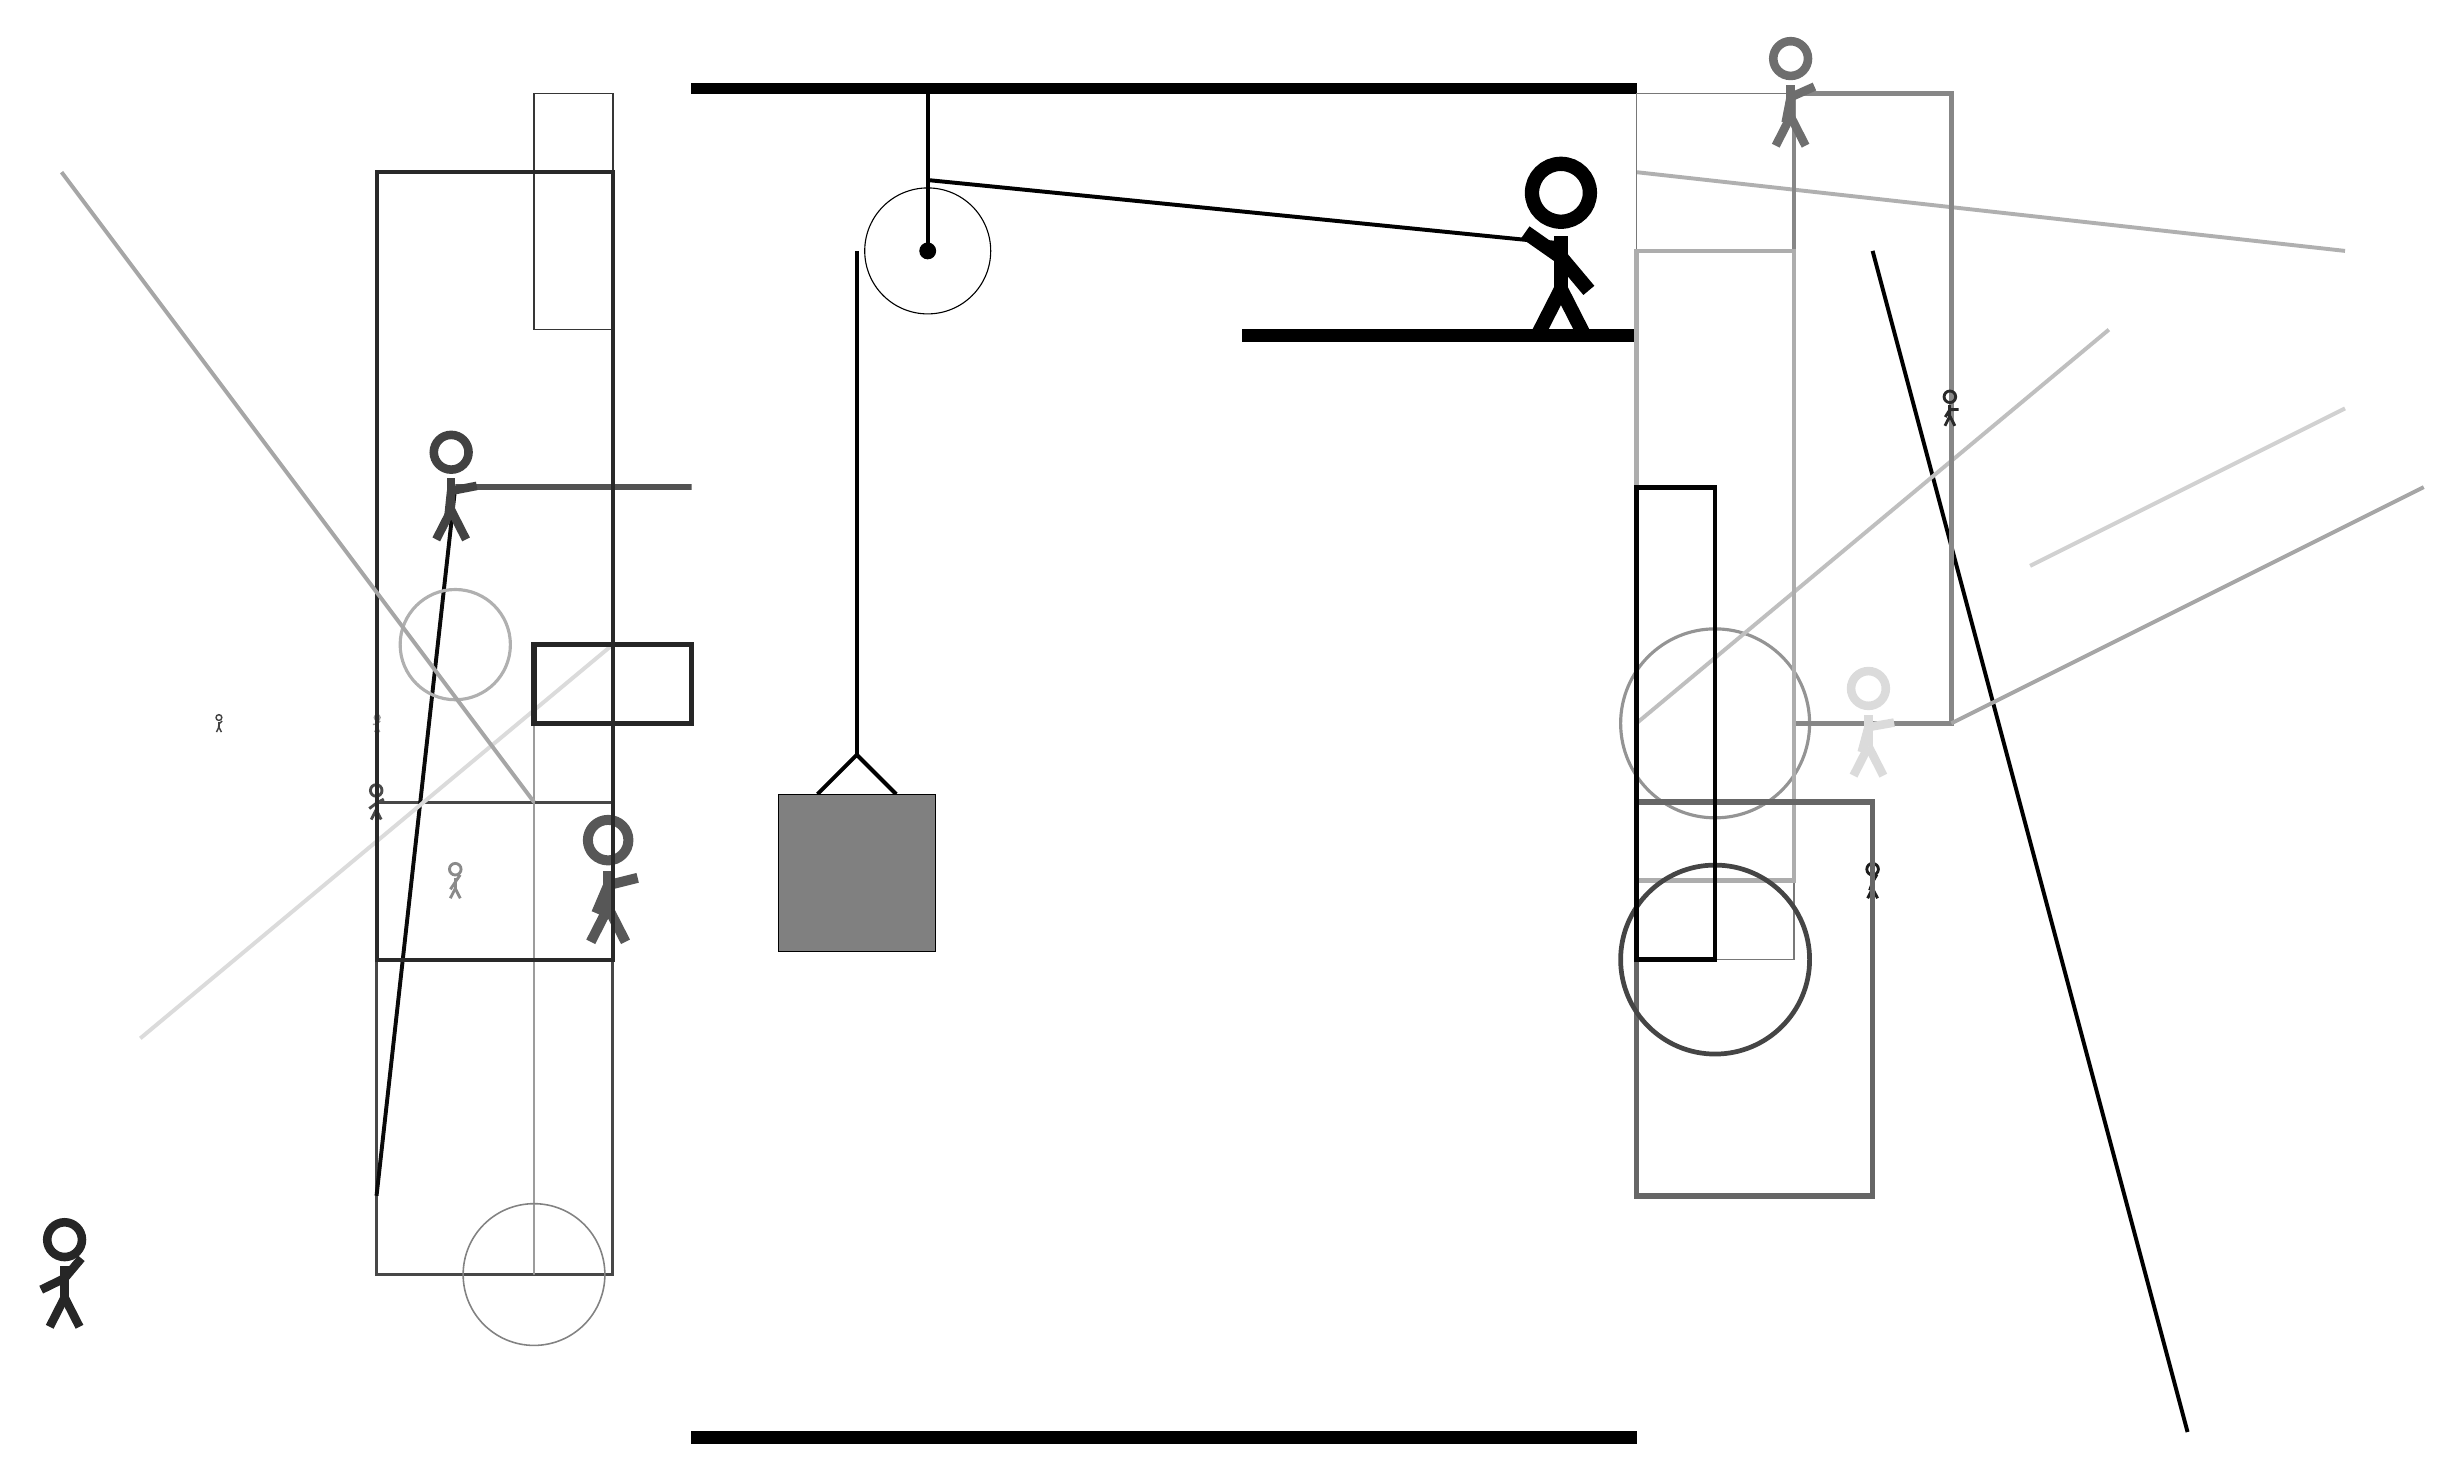
\begin{tikzpicture}
			%%%%% START %%%%%
			
			\draw[fill=black] (-2, 14) rectangle (10, 14.125);
			
			\draw (1, 12) circle (0.8);
			\draw[fill=black] (1, 12) circle (0.1);
			\draw[line width=0.5mm] (1, 14) -- (1, 12);
			
			\draw[line width=0.5mm](-0.4, 5.1) --  (0.1, 5.6) -- (0.6, 5.1);
			\draw[fill=black!50] (-0.9, 5.1) rectangle (1.1, 3.1);
			
			\draw[line width=0.5mm](0.1, 12) -- (0.1, 5.6);
			\centerarc[line width=0.5mm](1, 12)(90:180:0.9)
			\draw[line width=0.5mm](1, 12.9) -- (9, 12.1);
			
			\node at (9, 12) {\Strichmaxerl[10][-35][-50]};
			\draw[fill=black] (5, 11) rectangle (10, 10.85);
			
			\node[line width=0.7mm, color=black!39] at (-6, 6) {\Strichmaxerl[1][6][47]};
			
			\draw[line width=0.5mm, color=black!31](10, 13) -- (19, 12);
			\draw [line width=0.4mm, color=black!42](11, 6) circle (1.2);
			\draw[line width=0.4mm, color=black!72] (-3, 5) rectangle (-6, -1);
			\draw[line width=0.2mm, color=black!39] (-4, -1) rectangle (-4, 7);
			\draw[line width=0.2mm, color=black!79] (-4, 11) rectangle (-3, 14);
			\draw[line width=0.2mm, color=black!53] (12, 3) rectangle (10, 14);
			
			\draw[line width=0.7mm, color=black!68] (-2, 9) rectangle (-5, 9);
			\node[line width=0.7mm, color=black!71] at (-6, 5) {\Strichmaxerl[2][37][29]};
			\draw[line width=0.5mm, color=black!96](-5, 9) -- (-6, 0);
			\draw[line width=0.5mm, color=black!100](13, 12) -- (17, -3);
			\draw[line width=0.5mm, color=black!25](10, 6) -- (16, 11);
			\node[line width=0.5mm, color=black!89] at (13, 4) {\Strichmaxerl[2][70][60]};
			
			\draw[line width=0.5mm, color=black!36](-6, 2) -- (-6, 2);
			\node[line width=0.2mm, color=black!66] at (-3, 4) {\Strichmaxerl[7][67][14]};
			\draw[line width=0.5mm, color=black!18](15, 8) -- (19, 10);
			
			\draw [line width=0.4mm, color=black!31](-5, 7) circle (0.7);
			\draw[line width=0.5mm, color=black!14](-3, 7) -- (-9, 2);
			\node[line width=0.6mm, color=black!74] at (-8, 6) {\Strichmaxerl[1][84][43]};
			
			\draw[line width=0.6mm, color=black!47] (12, 6) rectangle (14, 14);
			\node[line width=0.4mm, color=black!74] at (-5, 9) {\Strichmaxerl[6][84][11]};
			\draw [line width=0.2mm, color=black!49](-4, -1) circle (0.9);
			\node[line width=0.3mm, color=black!46] at (-5, 4) {\Strichmaxerl[2][56][56]};
			\node[line width=0.7mm, color=black!14] at (13, 6) {\Strichmaxerl[6][75][10]};
			\draw[line width=0.7mm, color=black!85] (-4, 6) rectangle (-2, 7);
			
			\draw[line width=0.5mm, color=black!84] (-3, 13) rectangle (-6, 3);
			\draw[line width=0.5mm, color=black!35](14, 6) -- (20, 9);
			\draw[line width=0.6mm, color=black!32] (10, 4) rectangle (12, 12);
			\draw[line width=0.5mm, color=black!35](-4, 5) -- (-10, 13);
			\node[line width=0.6mm, color=black!84] at (14, 10) {\Strichmaxerl[2][58][1]};
			\draw[line width=0.7mm, color=black!60] (10, 5) rectangle (13, 0);
			
			\node[line width=0.4mm, color=black!85] at (-10, -1) {\Strichmaxerl[6][26][50]};
			\draw [line width=0.6mm, color=black!73](11, 3) circle (1.2);
			
			\draw[line width=0.6mm, color=black!99] (10, 3) rectangle (11, 9);
			\node[line width=0.7mm, color=black!57] at (12, 14) {\Strichmaxerl[6][79][24]};
			
			\draw[fill=black] (-2, -3) rectangle (10, -3.15);
			
			%%%%% END %%%%%
		\end{tikzpicture}
	\end{figure}	
\end{document}